The content-based recommender design section is split into a theoretical approach and a mathematical approach.

\subsubsection{Making the content-based recommender theoretically}

According to \cite{RecSysHandbook} the recommendation process is performed in three steps:

\subsubsection{Analyzer}

The first step towards a recommendation is to translate the items, from which the recommendations will be drawn, into a structured representation of the item. The source can either be documents, web pages, news or product descriptions. Extracting features of a movie or other media is straightforward, but when presented with documents a more complex process of finding high value words is needed. This will not be further discussed in this report.    
 
\subsubsection{Profile learner}

Next a similar process has to be made for the user. Data representative of the user has to be collected and translated into a similar structured representation. A users reactions, representing the items relevance, toward specific items has to be collected and stored. Those reactions together with the items, from which they are collected, are then used to construct the profile. The reactions could either be collected through automatic personalization or customization as described in Section \ref{Background} on page \pageref{Background}. Normal relevance information collected can either be:

\begin{description}
\item[Boolean] When users like/dislike items.


\item[Ratings] When users rate the items. E.g. on a scale from 1 to 10.


\item[Text comments] As used by Amazon.com when they request customer feedback on items. Other users can then later read the comments made by previous customers. The customization has the advantage of being more simplistic but at the same time requires more actions from the user. The automatic personalization does not require active user feedback but can get biased information when the user is interrupted in the middle of a session from outside influences like a phone call.
\end{description}

\subsubsection{Filtering component}
At the last stage the user profile is matched with item representations and a relevance list is made with most to least relevant items. The top listed items the user has not already consumed can then be recommended to him or her.
 
\subsubsection{Making the content-based recommender mathematically}

\subsubsection{Content analyzer}
- Making the Item profile:
 
According to \cite{MoMDatasets} an item can be represented with a vector of 0's and 1's where each spot in the vector corresponds to an associated person, a genre or other feature. If a specific actor is staring in the movie it gets a 1 in the spot corresponding to that actor and 0's in spots corresponding to actors not in the movie. The vector can also implement non-boolean values if a movies average rating is included. E.g. from IMDB.com using 1 to 10 scale rating system. But when using non-boolean values the scaling has to be considered. A rating of value 8 has a much higher weight than a "like"-value of 1.

\begin{figure}[H]
\centering
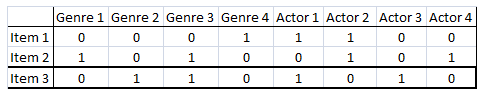
\includegraphics[width=0.8\textwidth]{Images/Vectorrepresentationitems.png}
\caption{Shows features and items}
\label{VrepItem}
\end{figure}

An example of 3 items are shown in \ref{VrepItem}. The entire row for item 3 becomes its vector representation where each position represents a specific feature.  
 
\subsubsection{Profile learner}
- Making the user profile:

We need to create matching vectors for the users with the same components so that a users vector and an item vector can be compared. But the user vector will not be made with booleans as they are too simple here. If we look at movies again there are 2 ways to make the vector. The simplest solution is, if a actor has been in 20\% of the movies seen by a user, the movie gets a 0.2 in the spot corresponding to that actor.

\begin{figure}[H]
\centering
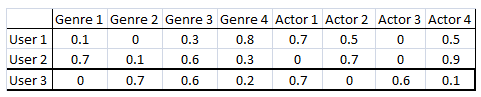
\includegraphics[width=0.8\textwidth]{Images/VectorrepresentationUsers.png}
\caption{Shows users and features}
\label{VrepUser}
\end{figure}

As shown in Figure \ref{VrepUser}, user vector representations are very similar to those of the items. The only change is the values and it is now possible to compare item 3 from Figure \ref{VrepItem} with user 3 to get a relevance judgment.

But a more precise solution is to take into account what rating the user gave the movies the before mentioned actor was in. The ratings can be further normalized from the users average rating by subtracting the average rating from the specific rating.

Example:

User 1 gives an average rating of 3, across all the items he has rated and has rated the 3 movies from before 3, 4 and 5. This can be seen in Figure \ref{Feature1}.

\begin{figure}[H]
\centering
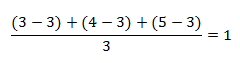
\includegraphics[width=0.4\textwidth]{Images/Userfeature1.png}
\caption{User 1 feature value}
\label{Feature1}
\end{figure}

User 2 gives an average rating of 4 and has rated 3 movies 2, 3 and 5. This can be seen in Figure \ref{Feature2}.

\begin{figure}[H]
\centering
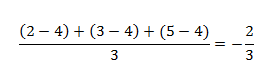
\includegraphics[width=0.4\textwidth]{Images/Userfeature2.png}
\caption{User 2 feature value}
\label{Feature2}
\end{figure}

This way it is possible to get negative values for actors starring in movies the user does not like.

 
\subsubsection{Filtering component}

Now with the vector representations for items and for the user, the relevance of an item can be computed as the angle between the item and the user vector using the cosine distance algorithm. It is worth noting that the cosine distance algorithm isn't affected by 0's corresponding to e.g. a genre the movie does not have. The cosine distance is calculated from the dot-product divided by the multiple of the lengths of each vector. This can be seen in Figure \ref{Cosine}.

\begin{figure}[H]
\centering
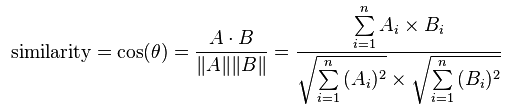
\includegraphics[width=0.8\textwidth]{Images/Cosinesimularity.png}
\caption{Cosine distance formula, from \ref{cosSimWiki}
\label{Cosine}
\end{figure}

If the more precise solution is used to generate the user profile from which we compute the cosine distance, for movies with many features (e.g. actors, genres) the user likes, get a large positive fraction implying an angle close to 0. When compared with items with a good spread of liked features and disliked features we will get a cosine distance close to 0 implying an angle close to 90 degrees and for the items with a lot of disliked features the cosine distance will be a large negative fraction implying an angle close to 180 degrees.